\synctex=1
\documentclass[a4paper,11pt]{article}
\usepackage[utf8]{inputenc}
\usepackage{graphicx}
\usepackage[a4paper, total={6.5in, 9in}]{geometry}
\usepackage{natbib}

\usepackage{nameref}
\newcommand*{\qref}[1]{\hyperref[{#1}]{\textit{``\nameref*{#1}'' (section \ref*{#1})}}}
\newcommand*{\qrefP}[1]{\hyperref[{#1}]{\textit{``\nameref*{#1}'', section \ref*{#1}}}}
\newcommand*{\qrefS}[1]{\hyperref[{#1}]{section \textit{\ref*{#1},
      ``\nameref*{#1}''}}}

\usepackage{hyperref}

\hypersetup{
  colorlinks = true,
  citecolor=  black,
  linkcolor = {blue},
  filecolor = cyan %% controls color of external ref, if used
}
\title{EvAM-Tools: additional documentation}
% \author{Ramon Diaz-Uriarte, Pablo Herrera-Nieto}

\author{Ramon Diaz-Uriarte\,$^{\text{\sfb 1,}}$, Pablo Herrera-Nieto\,$^{\text{\sfb 1}*}$}

\address{$^{\text{\sf 2}}$Department of Biochemistry, Universidad Autonoma de Madrid, Instituto de Investigaciones Biome´ dicas ‘Alberto
Sols’ (UAM-CSIC), Madrid, Spain}

\corresp{$^\ast$To whom correspondence should be addressed.}


\begin{document}



\begin{titlepage}
\maketitle
\tableofcontents
\end{titlepage}

 
% \section{Cancer progression models}
% The CPMs included are: 
% \begin{enumerate}
%     \item \textbf{Oncogenetic Tress (OT):} this is the simplest graphical model. Restrictions are represented as a tree. Hence, a parent node can have many children, but children have a single parent.
%     \item \textbf{Conjuntive Bayesian Networks (CBN):} this model generalizes the tree-based restricion of OT to a direct acyclic graph (DAG). A DAG allows to include multiple parents. In CBN, when a node depends of many parent events, all of the them have to be present for the children to appear. In that sense, CBN models this relationships as conjuntive, in other words, it models the AND relationship.
%     \item \textbf{Monte Carlo CBN (MCCBN):} this is an implementation of CBN using Monte Carlo expectationi-maximization algorithm to work with a large number of mutations.
%     \item \textbf{Progression Models of Cancer Evolution (PMCE):} is also a graphical model which main features it the aumatic detection of logical formulas AND, OR and XOR.
%     \item \textbf{Mutual Hazard networks (MHN):} in this model dpeendencies are not deterministic. In that sense, we do not see a direct dependence relationship, i.e. mutation B depends on mutation A. Conversely, an envent is influenced by all others. So, one event can make other more like (the presence of A promotes B) and also inhibiting it (the presence of A inhibits B). Hence, MHN includes multiple dependencies and is not limited to DAG schemes. The main parameters is a theta matrix that represents how one event influences other.
%     \item \textbf{Hypergraph Transition Path Sampling (HyperTraPS):}
% \end{enumerate}



% \section{Naming data, saving data}

\section{Building the models and example data}
\label{sec:build-models-example}

\subsection{Example data/DAGs/MHNs}
\label{sec:exampe-datadagsmhns}

For each of the ways to input cross-sectional data or build models, we provide some pre-built examples. You can use these to directly run the CPMs or modify them to your liking. The MHN and DAG builders allow you start from working examples. Explanations on what is available and why: 

\begin{description}
\item[Modifying pre-built examples] If you modify the examples, you probably will want to give your dataset or example a distinctive name.

\item[Modifying pre-built examples] If you modify a pre-built example and want to go back to the original, in your browser clean the cache and refresh.
  
\item[Cross-sectional data] We provide data sets that have been generated under specific models with AND, OR, XOR. However, no DAG is shown here, and that is on purpose; use the labels as possible hints, not as the truth and compare with datasets you can generate from models you specify under the DAG builder.

\item[DAG] 
  
\end{description}


\section{Cross-sectional data input}
\label{sec:cross-sectional-data}

\subsection{Number of genes and genes without mutations}
\label{sec:number-genes-genes}

 When creating user data (for instance, when adding new genotypes), any gene that has no mutations is automatically excluded from the data, regardless of the setting for number of genes. This is a feature, not a bug. For example, suppose you set the number of genes to 3, but you only specify frequencies, or counts, for genotypes "A" and "A, B". The data set will only contain columns for genes A and B (since gene C has no mutations and it would be excluded during the analyses).


\section{Generating random CPM/EvAM models, sampling from them, and error models}\label{sec:random_evam}


\subsection{Generating random CPM/EvAM models and sampling from them}\label{subsec:random_evam}
We often want to generate data under the model of a CPM. Common use cases are:

\begin{itemize}
\item Understand what different models imply about how the cross-sectional data looks like.

\item Examine how well a method can recover the true structure when the data fulfills the assumptions of a method. For instance, we would generate data under a particular model and see if the method that implements that model can recover the true structure under different sample sizes.

\item Examine how a give method works, and what type of inferences it performs, when data are generated under the model of another method. For example, what is the output from MHN if the data are really coming from an H-ESBCN model?
\end{itemize}


Addressing the above needs involves:


\begin{enumerate}
\item Generating random a model.
 
\item Obtaining the predicted genotype frequencies from that model.
 
\item Obtaining a finite sample from the predicted frequencies of that model.
  
\item Using the data to answer whichever questions we had; for example, analyzed the sampled data with another or the same method, plot the genotype frequencies, etc.
  
\end{enumerate}



We explain in each one in turn in details below, with reference to \texttt{evamtools} functions and arguments.

\begin{enumerate}
\item Generating a random model.
  
  Function \texttt{generate\_random\_evam} generates random models for OT, OncoBN, CBN, MHN, OncoBN, and H-ESBCN. Details about the arguments of the function are provided in its help page. No specific provision is made for randomly generating from MCCBN, as the way to simulate is similar to CBN (generate a random poset and a random set of lambdas).

\item Obtaining the predicted genotype frequencies from that model.
  
  These are returned as part of the output of \texttt{generate\_random\_evam} (as well as part of the output of \texttt{evam}). In all cases, the predicted distribution of genotypes for a model is done assuming perfect compliance with the model (see further details below).

\item Obtaining a finite sample from the predicted frequencies of that model.

  As the output from \texttt{generate\_random\_evam} is the same (except for the data components) to that from \texttt{evam} we can pass the model to function \texttt{sample\_CPMs}.

  When obtaining a finite sample, we can add sampling noise to the data. For example, noise due to genotyping errors; the probability of errors is controlled by argument \texttt{obs\_noise} in the call to \texttt{sample\_CPMs}.

  In more detail, the process involves:
  \begin{enumerate}
  \item Obtaining a finite sample without errors from the predicted genotype frequencies.
  \item If requested (i.e., if \texttt{obs\_noise > 0}), flipping a fraction \texttt{obs\_noise} of the observations (i.e., turning 1s to 0s and 0s to 1s).
  \end{enumerate}
  
\item Using the data to answer whichever questions we had; for example, analyzed the sampled data with another or the same method, plot the genotype frequencies, etc.

  To make this simpler, function \texttt{sample\_CPMs} can return the finite sample (with or without observation noise) as a typical cross-sectional data set: a matrix where each row is a "sampled genotype", in which 0 denotes no alteration and 1 alteration in the gene of the corresponding column. This data matrix can be used directly as input for CPM methods, for instance as argument \texttt{x} (the cross-sectional data) to function \texttt{evam}.

  
\end{enumerate}


\subsection{Error models}
\label{error_models}

We explained above that when obtaining the predicted frequencies under a model we assume perfect compliance with the model. This is straightforward with most methods, but not with others. This summarizes the error models for each method:

\begin{description}
\item[CBN] In H-CBN the $\lambda$s describe the true underlying model that produces the true, hidden genotypes, but the observed genotypes might differ from the true ones because of observation error, for instance genotyping error  \cite[p.~2810]{gerstung2009quantifying}.
\item[H-ESBCN] As for CBN \cite[p.~756]{angaroni2021}.
\item[MHN] As for CBN (e.g., description of the simulation process in p.244 of \citealp{schill2020modelling}).
\item[MC-CBN] With MC-CBN the model is mixture between the CBN model and a noise component model \cite[p.~i730-i731]{montazeri2016large}. The simulations in \url{https://github.com/cbg-ethz/MC-CBN}, however, use a procedure where observations are generated from an underlying poset with a given set of lambdas, and symmetric error is then added (see the functions \texttt{mccbn:::random\_poset} and \texttt{mccbn:::random\_posets}).
\item[OncoBN] The model includes a DBN (disjunctive) or CBN (conjunctive) model, as given by a DAG and a set of $\theta$s, and an ``spontaneous activation model'' \cite[p.~3-4]{nicol2021oncogenetic}. The ``spontaneous activation model'', with parameter $\epsilon$, represents deviations from the DBN or CBN and allows child mutations to appear even if the parents in the DAG have not been mutated (i.e., even if the DAG restrictions are not satisfied).
  
\item[OT] There are two sources of deviations from the OT model: a) those that result from observational (or genotyping) errors, that can lead to both false positive and false negative observational errors; b) events occurring that do not respect the OT model \cite{Szabo2002}. The second would be the same as the ``spontaneous activation'' in OncoBN.
  
  The \texttt{oncotree.fit} function in the \texttt{Oncotree} package returns a \texttt{eps} component with the estimated false positive, \texttt{epos}, and false negative, \texttt{eneg}, error rates. But these are the result of combining the two sources of error \cite{Szabo2008}: observation errors and true deviations from the model. So observation error is reflected in both \texttt{eneg} and \texttt{epos}, whereas true deviations from the model are only reflected in \texttt{epos}. In other words, the false negatives, as measured by the estimated  \texttt{eneg}, are due purely to observation error. But the \texttt{epos} are not equivalent to the $\epsilon$ of OncoBN: \texttt{epos} includes both observation error (false positives) and true mutations that occur without respecting the restrictions of the OT DAG (tree). 
  
\end{description}


\subsection{Error models and simulating and sampling from OT}
\label{error_ot}
Given the above, when sampling from a model, in all cases except OT, we have always followed the same procedure:  we have first generated observations under the true model and, if requested, then added noise. For OT, since \texttt{epos} reflects both observation and true deviations from the model, this is not possible. Thus, for OT there is a difference when we sample from a random model and when we sample from the predictions of a fitted model.

The fitted model for OT, when fitting a true data set, includes both \texttt{epos} and \texttt{eneg}. Predictions are obtained using function \texttt{Oncotree::distribution.oncotree} with, by default, argument \texttt{with.errors = TRUE}, which is what argument \texttt{with\_errors\_dist\_ot = TRUE} to \texttt{evam} does. Therefore, from a fitted model, the predictions incorporate both false positive and false negative error rates, as estimated by \texttt{oncotree.fit}; as explained above, however, these estimated error rates are both the errors from the observational process (genotyping errors, for example) and true deviations from the model. When you later call \texttt{sample\_CPMs} you can add an \texttt{obs\_noise} with value larger than 0, but for OT, when sampling from the model fitted to observed data this might not make sense (since \texttt{epos} and \texttt{eneg} have been used already to produce the predicted genotype frequencies). Thus, if we use \texttt{with\_errors\_dist\_ot = TRUE} in the \texttt{evam} call and then set \texttt{obs\_noise = 0} when calling \texttt{sample\_CPMs}, the observed data we generate should be the same (have the same distribution) as if we had used \texttt{Oncotree::generate.data} with \texttt{method = ``D1''}, \texttt{with.errors = TRUE} and \texttt{edge.weights = ``estimated''}.\footnote{
  We can try to divide the \texttt{epos} component in a component like OncoBN's $\epsilon$ and another noise component. Then, we would first obtain the predicted distribution via \texttt{distribution.oncotree} with the $\epsilon$-like (and with \texttt{eneg} = 0), sample, and add noise. If \texttt{epos} $>$ \texttt{eneg} we can do this so that the noise added is symmetrical. This is shown in function \texttt{dot\_noise\_gd\_3} in \texttt{inst/miscell/OT\_generate\_data\_sample\_CPMs.R}.

  
In that same file \texttt{inst/miscell/OT\_generate\_data\_sample\_CPMs.R} we show that a model obtained from \texttt{generate\_random\_evam} with \texttt{ot\_oncobn\_eps}  $= x$ and sampled using \texttt{sample\_CPMs} with \texttt{obs\_noise} $= y$ gives predictions with the same distribution as if we had used \texttt{Oncotree::generate.data} on that very same oncotree object but with \texttt{epos} = $x + y - (1/2)\ x\ y$ and \texttt{eneg} = $y$.}



When sampling from a random model, using \texttt{generate\_random\_evam}, we generate the tree (the DAG) with density as given by argument \texttt{graph\_density} and the weights from uniform distributions with limits  given by \texttt{ot\_oncobn\_weight\_min} and \texttt{ot\_oncobn\_weight\_max}. In addition, we can set a value larger than 0 for \texttt{ot\_oncobn\_epos}. This will be used as the \texttt{epos}, but not \texttt{eneg}, value of the OT model. When you sample and optionally add noise, with argument \texttt{obs\_noise} to function \texttt{sample\_CPMs} noise is added symmetrically. Thus, we use a procedure where \texttt{ot\_oncobn\_epos} behaves as OncoBN's $\epsilon$ and \texttt{obs\_noise} is purely symmetric observational error.


Why this difference? When you use a model fitted to real data, it is sensible to use \texttt{Oncotree}'s inferential machinery to estimate the \texttt{epos} and \texttt{eneg}. If you later want to generate samples, these already include deviations from the model and noise. However, when you simulate a model, there is no data and thus no way to estimate the \texttt{epos} and \texttt{eneg}. Therefore, it is sensible to split errors into two distinct pieces, which is also coherent with what we do with the rest of the methods: deviations from the model, and noise.



%% I only understand the meaning of a few combinations:
%% D1 and D2, these are the equivalent calls.
% d1 <- generate.data(3e5, ov.tree, with.errors = TRUE, method = "D1",
%                     edge.weights = "estimated")
% d3 <- generate.data(3e5, ov.tree, with.errors = TRUE, method = "D2",
% edge.weights = "estimated")


%% So with errors, D2, estiamted, which calls dist.oncto w/o errors, but using estimated, and then adds the errors.

%% The thing is that distribution.oncotree uses, correctly, the errors. 




\section{Random EvAM models and transitive reduction}
\label{sec:random-evam-models}

As of now, the generation of random EvAM models uses transitively reduced graphs (we call \texttt{mccbn::random\_poset} with argument \texttt{trans\_reduced = TRUE}). This does not decrease the number of models that can be expressed when using CBN. However, it can limit the range of models when we can mix AND, OR, XOR in the same model. The following  examples illustrate how this makes certain models impossible.

\begin{figure}[h!]
\centering
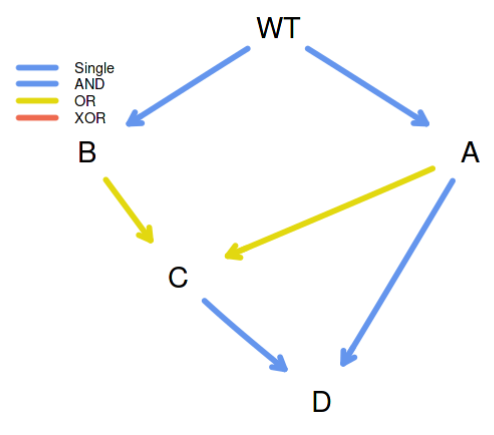
\includegraphics[width=.23\linewidth]{./dag2.png}
\caption{Non-transitively reduced DAG, OR and AND}\label{dag2}
\end{figure}

Under DAG in Fig.~\ref{dag2} we cannot observe genotype BCD.

\begin{figure}[h!]
\centering
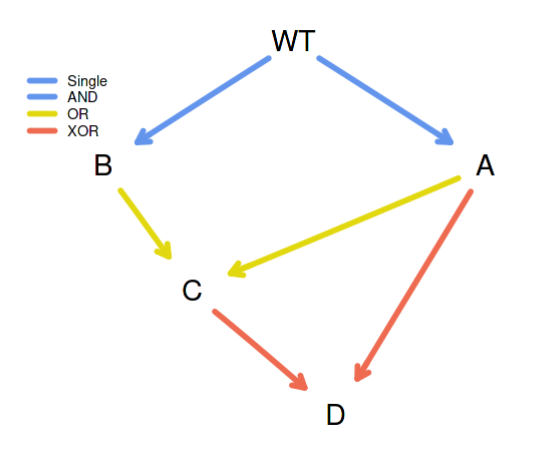
\includegraphics[width=.23\linewidth]{./dag3.png}
\caption{Non-transitively reduced DAG, OR and XOR}\label{dag3}
\end{figure}

Under DAG in Fig.~\ref{dag3} we cannot observe genotype ACD.


\begin{figure}[h!]
\centering
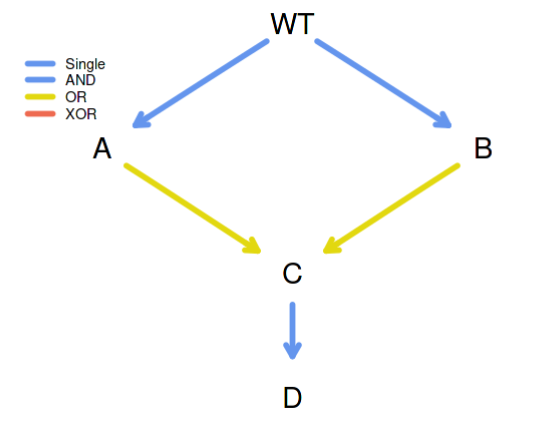
\includegraphics[width=.23\linewidth]{./dag1.png}
\caption{Transitively reduced DAG}\label{dag1}
\end{figure}

Under DAG in Fig.~\ref{dag1}, which is the transitive reduction of the above two graphs, we can observe both BCD and ACD.

Can we imagine biological scenarios where Fig.~\ref{dag2} or Fig.~\ref{dag3} would apply? Yes. We don't recall seeing them in the literature, though. If this is deemed relevant, it is just a matter of changing  \texttt{trans\_reduced = TRUE} when we are simulating HESBCN models inside function \texttt{random\_evam}.

You can of course construct the non-transitively reduced graphs by hand or using the shiny app.









% \section{Sampling scheme}
% From transition rate matrices it is possible to establish a scheme to sample a population based on stochactic simulation with continious time Markov chains \cite{wilkinson2018stochastic}.

% To sample an individual the proccess include the following steps:
% \begin{enumerate}
%   \item SET \textit{sample time}. It is drawn from an Exp($\lambda = 1$). This is the time at which the observation will be made, and when the sampling process will finish. 
%   \item \textit{Accumulated time} SET to zero.
%   \item SET \textit{trajectory} to wild type (no genes is mutated).
%   \item WHILE \textit{accumulated time $<$ random sampling time AND
%    having accesible genotypes}:
%    \begin{enumerate}
%        \item \textit{Time until next mutation}. It is defined with competing exponentials. It is decided by taking the minimun time from random samples with the rates of each accesible genotype. 
%        \item IF: \textit{acumulated time $+$ time until next mutation $<=$ sample time}:
%        \begin{enumerate}
%            \item ADD new mutation to the \textit{trajectory}.
%        \end{enumerate}
%        \item ELSE: \textit{end sampling}
%    \end{enumerate}
% \end{enumerate}


% \section{Validation of the sampling algorithm}

% Our implementation for sampling from transition rate matrices has been validated by comparing genotypes frequencies from our sampling scheme against to other implementations provided with the packages of MCCBN and MHN:

% For a single comparison we generated random data for either MCCBN and MHN.
% We then made a sample of 100 000 individuals with both the native software (either MCCBN or MHN) and with our implementation (after deriving the transition rate matrix).
% This yield two sets of observed genotypes that were compared with a Chi-Squared test to test whether both observed distributions came from the same underlying probability distribution.  
% P-values are expected to follow a uniform distribution Figures \ref{SI:MHN} and \ref{SI:MCCBN}.

% The above test was performed for data sets with 5, 6, 7, and 8 genes.
% For each gene, 10 000 random data were generated and with each population containing 100 000 individual samples.

% For ks test, recall we are using permutation test, so min p.value is not but 1/(B + 1).

% Scripts for running all samples and to compare them can be found in: 

% % \texttt{https://github.com/PabloHNieto/CPM-SSWM-Sampling/tree/tupac/guloMAM/insts/miscell/tests-sample_genotypes_from_trm}

% % \begin{enumerate}
%   %     \item Random data generation: with native code from MHN or MCCBN. (Include number of genes tested, number of examples per gen, and number of samples per run.)
%   %     \item Sampling process with native code based on random data.
%   %     \item Compute observed genotype frequencies from sampling with native code.  
%   %     \item Derived transitions rate matrices from random code with guloMAM.
%   %     \item Sampling process with guloMAM sampling code.
%   %     \item Compute observed genotype frequencies from sampling with guloMAM.
%   %     \item Compare distributions with chi-squere test and Kolmogrov-Smirnov test.   
%   % \end{enumerate}    
  
%   % P-values for each test are expected to follow a uniform distribution (ref to figure and table).
%   % Code and results for this is found in \dots 
  
%   % \begin{figure}
%   %   \centerline{
%   %     \includegraphics[]{"MHN.png"}
%   %     }
%   %   \caption{\textbf{MHN vs guloMAM sampling}. Distribution of p-values from Chi Square Test comparing genotype distribuion from MHN sampling and guloMAM sampling. The blue line indicates the cumulative distribution for a uniform distribution. The black line represents the cumulative probability of observing a p value lower than a given value.
%   %   }
%   %   \label{SI:MHN}
%   % \end{figure}
  
%   % \begin{figure}
%   %   \centerline{
%   %     \includegraphics[]{"MCCBN.png"}
%   %     }
%   %     \caption{\textbf{MCCBN vs guloMAM sampling.} Distribution of p-values from Chi Square Test comparing genotype distribuion from MHN sampling and guloMAM sampling. The blue line indicates the cumulative distribution for a uniform distribution. The black line represents the cumulative probability of observing a p value lower than a given value.
%   %     }
%   %     \label{SI:MCCBN}
%   % \end{figure}
    
% \section{Hypergraph embedding}
% Adapted from \textit{Graph Embedding and Visualization for Dynamic Acquisition on the Hypercube}

% \textbf{ADD FIGURES OF A SIMPLE SAMPLING PROCESS SHOWING THE DAG AND THE HYPERGRAPH}
    




\section{Tabular output from the Shiny app}
\label{tabular-output}

\begin{description}
\item[Transition probabilities] Conditional probability of transitions to a genotype (obtained using competing exponentials from the transition rate matrix; for OT and OncoBN this is actually a abuse of the untimed oncogenetic tree model, as explained in \cite{diaz2019every}.
\item[Transition rates] Transition rates of the continuous time Markov chain that models the transition from one genotype to another. This option is not available for OT and OncoBN, as these do not return rates.
\item[Predicted genotype relative frequencies] The predicted frequencies of genotypes under the model. See \qrefS{error_models} for details about OT and OncoBN
\item[Sampled genotype counts] Counts, or absolute genotype frequencies, obtained by sampling from the predicted frequencies.
  
  %% Next only if you ask for 'Sample for observed genotype transitions'
\item[Observed genotype transitions (counts)] Only if you ask for 'Sample for observed genotype transitions' in the Advanced options. Number of observed transitions between genotypes.
  
\end{description}


See also further details in section \qrefS{error_models} as well as in the help for functions \texttt{evam} and \texttt{sample\_CPMs}.



\section{FAQ}
\label{sec:faq}

\subsection{With OncoBN sometimes I obtain DAGs that are not transitively reduced}

Yes, that can happen. See details here \url{https://github.com/phillipnicol/OncoBN/issues/5}.

\subsection{I want to setup my own Shiny server with different default ``Advanced options''}

In file \texttt{EvAM-Tools/evamtools/inst/shiny-examples/evamtools/ui.R} search for ``Advanced options'' and modify the defaults to whatever you want.


\subsection{In the DAG figures, why do nodes with two or more incoming edges have only a single annotated edge with a number?}
\label{faq-single-num}

Because the number, which is the $\lambda$ (CBN, HESBCN) or $\theta$ (OncoBN) is the rate (CBN, HESBCN) or probability, conditional on the assumptions indicated by the DAG being satisfied. So the $\lambda$ or $\theta$ are per node, not per edge. For instance, suppose gene C depends on both A and B (there is an AND); and you see a number of 0.7. That is the $\lambda$ or $\theta$ for observing C mutated when both A and B are mutated. 


And why then not annotate the nodes, instead of the edges? Because in our experience:
\begin{itemize}
\item Annotating nodes leads to more confusing figures.
\item Annotating edges shows what transitions are likely/fast, an idea not conveyed by annotating nodes.
\end{itemize}

\subsection{Do sampled genotype frequencies and counts contain observation noise? And predicted genotype frequencies?}
\label{sec:do-sampled-genotype}

For all models except OT, predicted genotype frequencies do not have observation noise added. The OT model itself estimates noise, and thus predicted frequencies obtained from models fitted to observed data incorporate observation noise. See \qref{error_models}.

When we obtain a finite sample from the predicted frequencies, you can decide to add observation noise with argument \texttt{obs\_noise} to function \texttt{sample\_CPMs}; what happens with OT depends on whether the predictions are from a simulated model or a model fit to observed data; see details in \qref{error_ot}.


\subsection{Using the Shiny app in a local intranet with load balancing using multiple Docker instances}
\label{haproxy}

This is well beyond the scope of this document and there are many options available. One that can work is the following:
\begin{itemize}
\item Start multiple Docker instances (say, 10) by changing the range of ports, for example 3010 to 3020.
\item Use HAProxy (\url{https://www.haproxy.org/}) so that you have a single entry point for all requests to the service that are then distributed, with load balancing, to the 10 instances. You will want to use ``sticky connections''.
\end{itemize}

As said above, this is just a sketch of the basic procedure. There are many other options.


\subsection{Why aren't you using Shiny Server?}
\label{sec:why-arent-you}

Because we did not see it as necessary or convenient. If you want to run Shiny interactively from an R session load \texttt{evamtools} and call function \texttt{runShiny}; no need for Shiny Server.

If we want to run Shiny as a service, with Docker images it is rather straightforward to launch a bunch Docker instances and use HAProxy to access to them using load-balancing (see \ref{haproxy}) or any other such similar solution.

Moreover, notice this in the Shiny Server documentation (\url{https://shiny.rstudio.com/articles/shiny-server.html}): ``Shiny Server will host each app at its own web address and automatically start the app when a user visits the address. When the user leaves, Shiny Server will automatically stop the app. ''  That is not exactly what we want. We want the containers to be up and running, ready to answer requests as they come with minimal latency. Moreover, a single Shiny Server would have given access to a single instance of the app (so that if two or more users access the app, one of the users has to wait while R is busy executing what the other user is running); to give users access to multiple simultaneous instances we would have needed, for example, multiple Docker images each with its own Shiny Server.

However, we might be missing something; if you think Shiny Server would allow or ease some use cases, please let us know.


\bibliographystyle{natbib}
\bibliography{cpm_refs}



\end{document}